\subsection{Splitting Auroral Arcs}\label{sec:split}
One of the ground-observable optical manifestations of a DAW event are bifurcating ``shedding'' or ``splitting'' arcs, which have a pattern of one or more spatiotemporal leaves folding off of the main arc. 
During the shedding event of Figures~\ref{fig:20130414T0854a}-\ref{fig:20130414T0854b}, PFISR power in the magnetic zenith beam (represented by a red circle in Figure~\ref{fig:20130414T0854a}(a-d)) is enhanced by over \unit[25]{dB} in the F-region ionosphere above the bifurcation zone.
\begin{sidewaysfigure}\noindent

    \includegraphics[width=\columnwidth,trim=0 680 0 50,clip]{gfx/2013-04-14T0854/2013-04-14T0854}\\
    
    \vspace{-1.175cm}
    \hspace{1.35cm}{\color{white}(a) 08:54:16}
    \hspace{2.1cm}{\color{white}(b) 08:54:21}
    \hspace{2.15cm}{\color{white}(c) 08:54:26}
    \hspace{2.15cm}{\color{white}(d) 08:54:31}
    \vspace{0.5cm}
    
    % backscatter
    \begin{center}
    \includegraphics[width=0.9\columnwidth,trim=10 0 0 185,clip]{gfx/2013-04-14T0854/power_longpulse2013-04-1408-54}\\
    \end{center}
    
    \vspace{-1.5cm}
    (e) 
    \vspace{.5cm}
      
    \caption{Splitting auroral arc sequence at PFISR, April 14, 2013. 
        (a) beginning of plasma turbulence bursts.
        (b) F-region ionization increasing nearly \unit[30]{dB} above background. 
        The turbulence fades in (c), enhancing to even greater intensity in (d) for ten seconds.
        (e) backscattered ISR power.}
    \label{fig:20130414T0854a}
\end{sidewaysfigure} 

\begin{figure}\noindent
	   % psd ion-line 
	\includegraphics[width=0.425\columnwidth]{gfx/2013-04-14T0854/acfslice_longpulse2013-04-1408-54-16}
	\includegraphics[width=0.425\columnwidth]{gfx/2013-04-14T0854/acfslice_longpulse2013-04-1408-54-31}\\
	
	\vspace{-1.5cm}
	\hspace{0.0cm}(a)\hspace{0.4\columnwidth}(b)
	\vspace{0.3cm}
	
	% down-shift
	\includegraphics[width=0.425\columnwidth,trim=0 50 0 0]{gfx/2013-04-14T0854/plasmaDOWNslice2013-04-1408-54-16}
	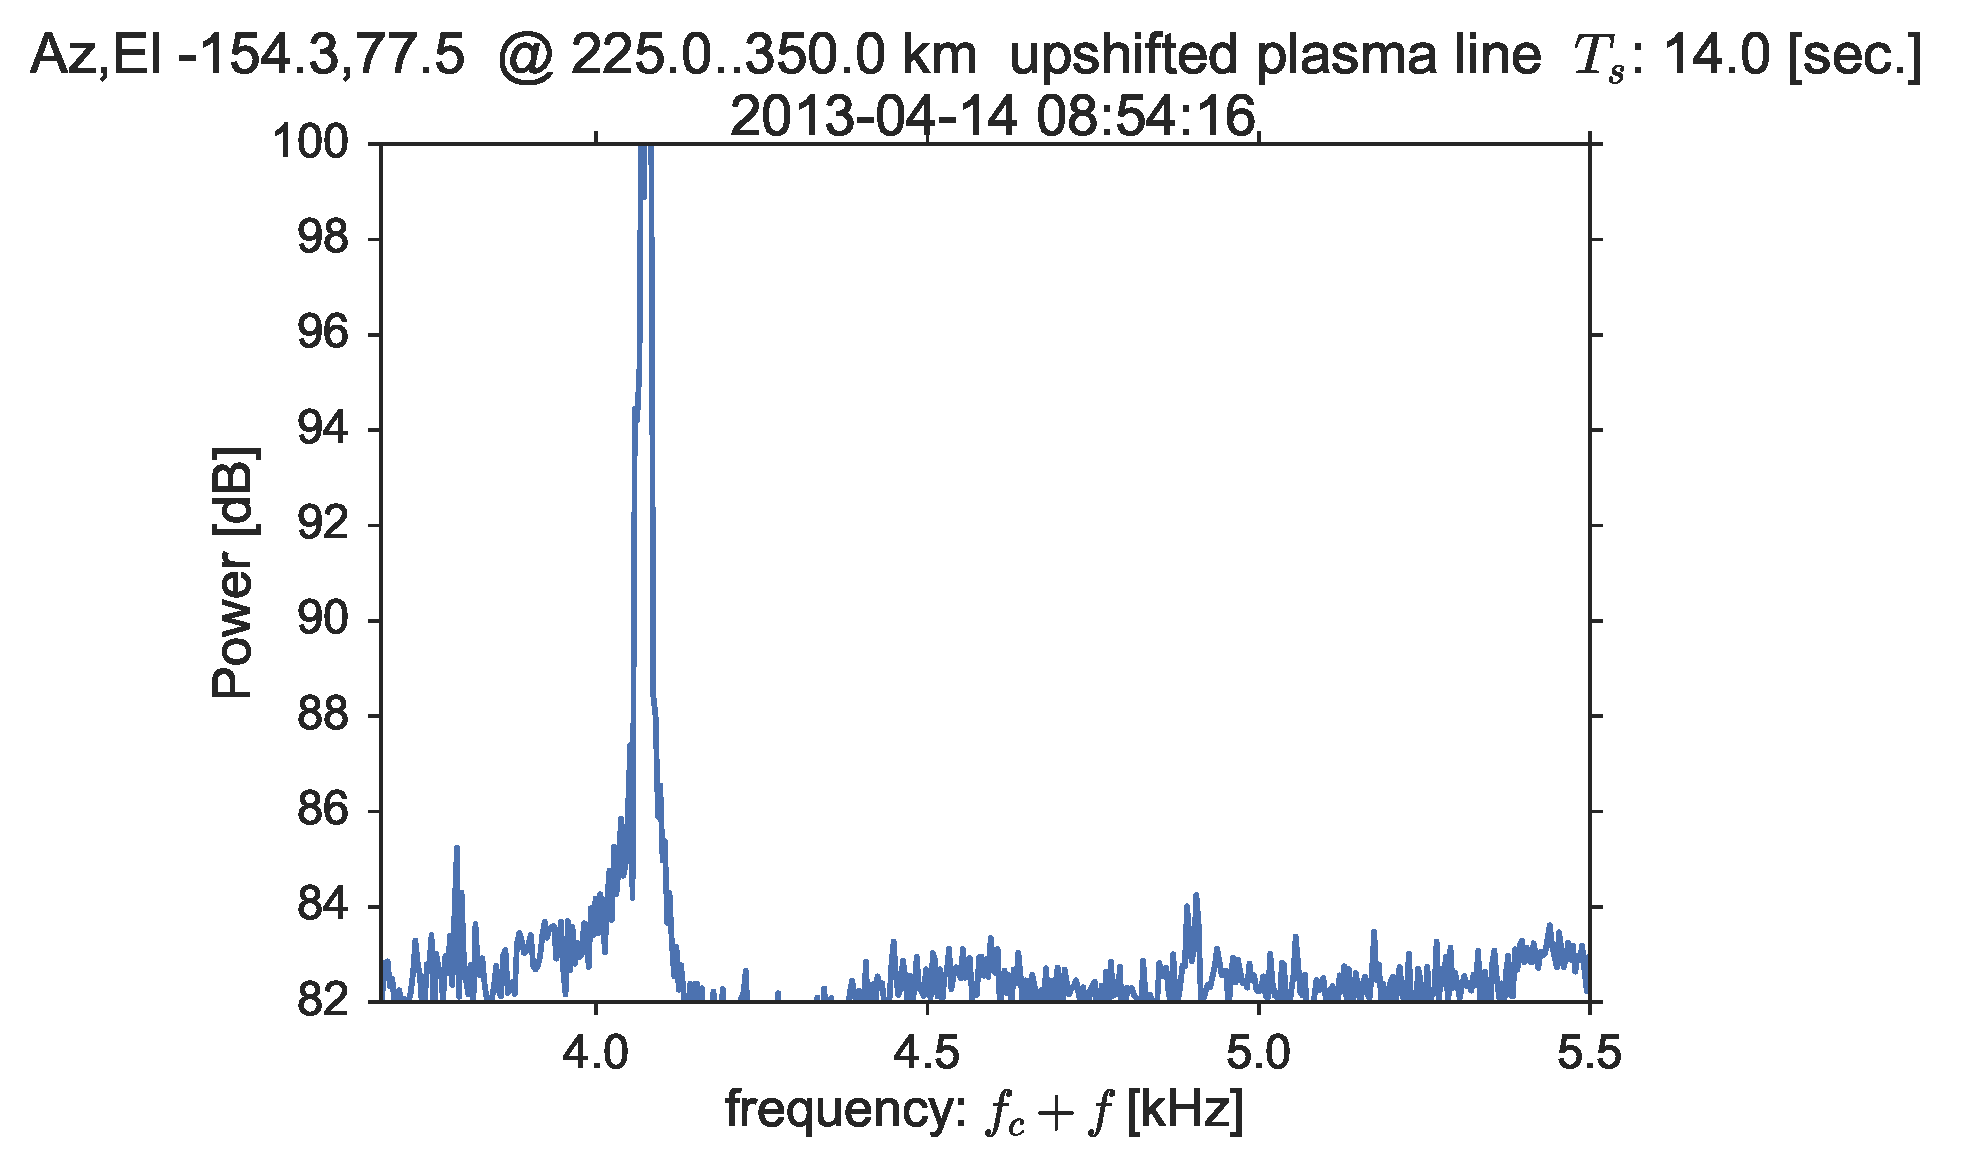
\includegraphics[width=0.425\columnwidth,trim=0 50 0 0]{gfx/2013-04-14T0854/plasmaUPslice2013-04-1408-54-16}\\
	
	\vspace{-1.2cm}
	\hspace{0.0cm}(c)\hspace{0.4\columnwidth}(d)
	\vspace{0.3cm}
	
	% up-shift
	\includegraphics[width=0.425\columnwidth,trim=0 50 0 0]{gfx/2013-04-14T0854/plasmaDOWNslice2013-04-1408-54-31}
	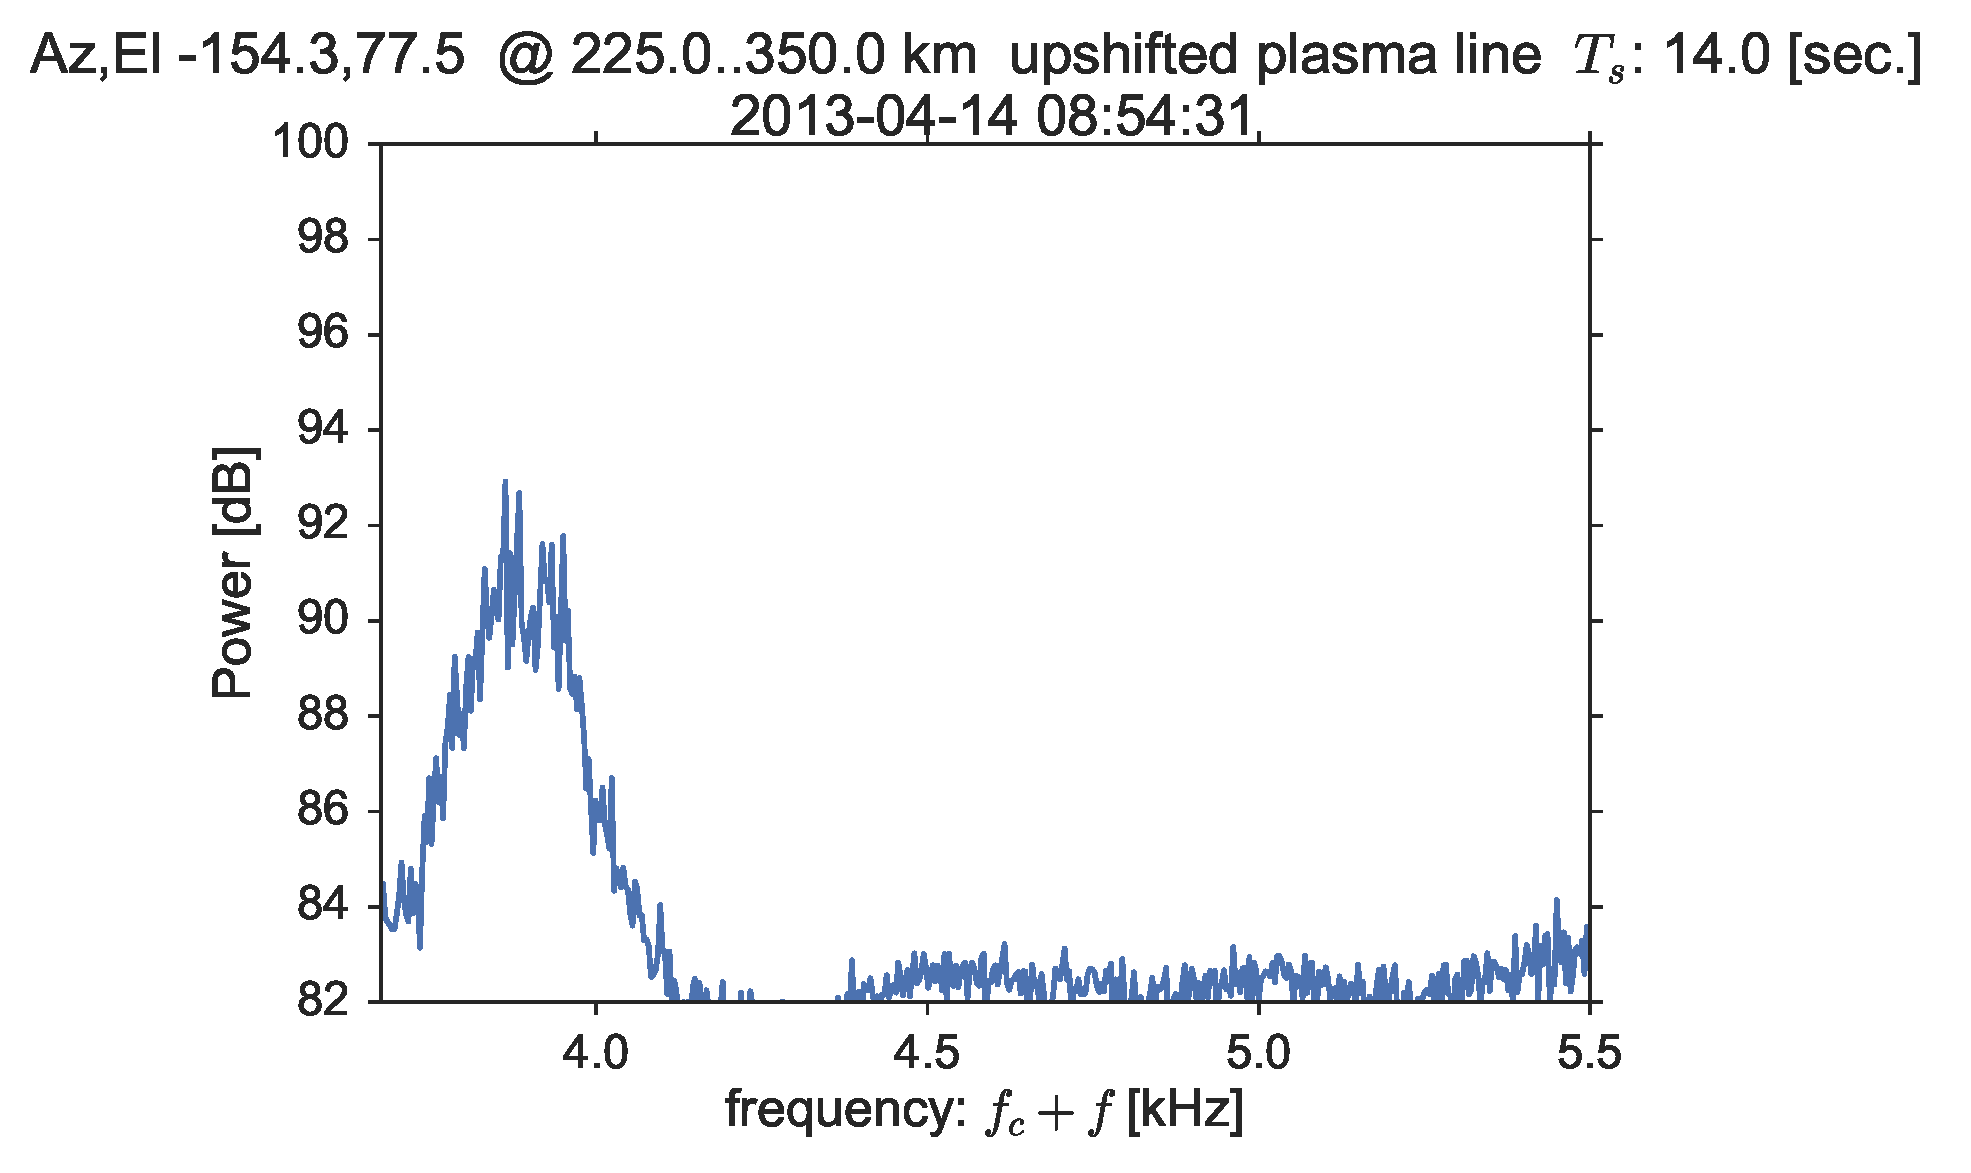
\includegraphics[width=0.425\columnwidth,trim=0 50 0 0]{gfx/2013-04-14T0854/plasmaUPslice2013-04-1408-54-31}\\
	
	\vspace{-1.2cm}
	\hspace{0.0cm}(e)\hspace{0.4\columnwidth}(f)
	\vspace{0.3cm}
	
	\caption{Splitting auroral arc sequence at PFISR, April 14, 2013.
		(a,b) backscattered power related to (a-c) and (d) respectively.
		(c,d) down- and up-shifted plasma line enhancements corresponding to Figure~\ref{fig:20130414T0854a}(a-c).
		(e,f) down- and up-shifted plasma line enhancements corresponding to Figure~\ref{fig:20130414T0854a}(d).}
	\label{fig:20130414T0854b}
\end{figure}
On the night of April 14, 2013, several instruments with diverse observing modalities were active in the vicinity of PFRR, as depicted in Figure~\ref{fig:sitemap}. 
PFISR and DASC are co-located, so the center of the PFISR beams in the image can be taken as approximately constant.
The GIMA magnetometer data is shown in Figure~\ref{fig:gima0854}, showing the usual southward IMF in the time vicinity of the splitting arc.
\begin{figure}
	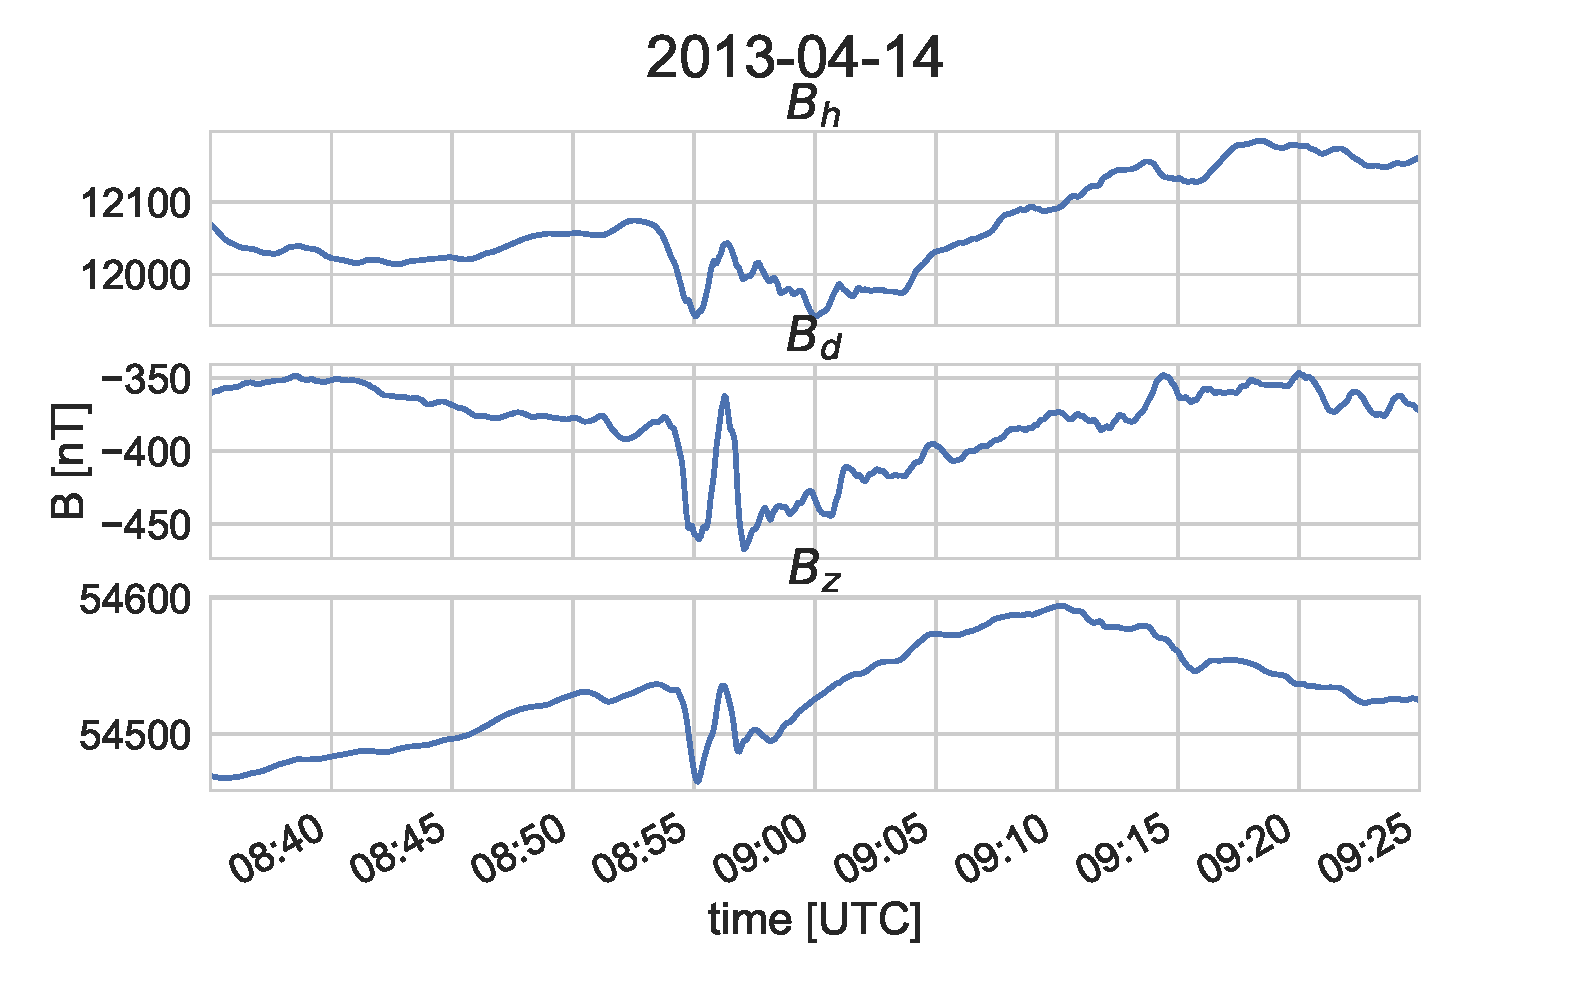
\includegraphics[width=\columnwidth]{gfx/2013-04-14T0854/mag}
	\caption{PFRR GIMA magnetometer data for 2013-04-14 showing evidence of southward IMF in time vicinity of splitting arc.}
	\label{fig:gima0854}
\end{figure}


Observe in Figure~\ref{fig:20130414T0854b}(c-f) that only the plasma line spectra for 08:54:16 and 08:54:31 UT show prominent reflections from plasma turbulence.
The rest of the plasma line spectra near this time looks much like the 08:54:45 data.
%In contrast, the ion line spectrum in Figure~\ref{fig:20130414T0854}(f,g,h) still shows the turbulence effects at 08:54:45, so an earlier frame at 08:54:02 UT is included to show the non-turbulent ion line spectra.
%A movie sequence for this event is available in the Supplemental Materials for this article.
We integrate the received ISR power over the NEIALs altitude range and plot this integrated measurement with the HiST optical data. 
It is initially apparent from comparing Figure~\ref{fig:20130414T0854a}(a-d) with Figure~\ref{fig:20130414T0854a}(e) that the highest SNR bursts come from the times when the magnetic zenith ISR beam is over a region of optically ``shedding'' arcs.
Figure~\ref{fig:20130414T0854a}(a) depicts a typical dispersive Alfvén wave auroral scene. 
The red circle denotes local magnetic zenith. 
Observe the fine spatial structure along the $B_\perp$ direction. 
Figure~\ref{fig:shedintion}(b) shows the plasma line summed over altitudes from \unit[200..350]{km}.
Figure~\ref{fig:20130414T0854b}(a,b) shows the ion line PSD during the time of this shedding auroral event--observe the ``flat top'' characteristic of the spectrum seen only during NEIALs.

Turning to optical spectral information, the PF-DMSP data in Figure~\ref{fig:shedratio0854}(a-b) is used to compare \unit[427.8]{nm} intensity from N$_2^+$ $I_{427.8}$ with prompt OI emissions at \unit[630.0]{nm} $I_{630.0}$.
This ratio in Figure~\ref{fig:shedratio0854}(c) shows that just before and during the splitting arc, $I_{427.8}$ is nearly twice as strong as $I_{630.0}$. 
\begin{figure}
    \includegraphics[width=\columnwidth,trim=3 3 3 3,clip]{gfx/2013-04-14T0854/MSPintensityratio}
    \caption{PF-DMSP (a) $I_{630.0}$ and (b) $I_{427.8}$ emission intensity with (c) $I_{630.0}/I_{427.8}$ emission intensity ratio at 08:54 UT during the 14 April 2013 substorm. Golden dashed lines refer to approximate elevation FOV of HiST cameras.}\label{fig:shedratio0854}
\end{figure}
After the splitting event completes, the \unit[630.0]{nm} line once again dominates $I_{427.8}$ by a factor of 1.5 to 3.5 as was also the case before the splitting began.
Figure~\ref{fig:shedratioplot0854} provides an alternative view of $I_{630.0}$/$I_{427.8}$.
\begin{figure}
    \includegraphics[width=0.9\columnwidth]{gfx/2013-04-14T0854/msp_ratio}
    \caption{PF-DMSP ratio of $I_{630.0}/I_{427.8}$ emission intensity ratio with one line plot per time. Observe that high energy beam (indicated by lowest ratio at 08:54:10) does not immediately lead to splitting arc. It takes about 10 seconds for visible arc splitting to occur. Golden dashed lines refer to approximate elevation FOV of HiST cameras.}
    \label{fig:shedratioplot0854}
\end{figure}
%These measurements are within the typical range for $I_{630.0}$ and $I_{427.8}$~\citep{Dashkevich2006}.
From \citet{rees1974}, at 08:54:10 UTC at the magnetic zenith angle of $102.5^\circ$ elevation from north, $I_{630.0}/I_{427.8} \sim 0.6$, corresponding to a characteristic energy of \unit[1.6]{keV} for the assumptions on neutral composition and brightness observed.

Historical work has often relied on spectrometer readings for estimates of characteristic energy $E_0$, represented in Figure~\ref{fig:alfvenflux} as the high-energy ``bump''.
Historically these measurements had cadences of several seconds, and obviously lacked a sense of the auroral morphology.
As the extensive literature referenced throughout this paper has noted, quantitative correlation of auroral spatio-temporal evolution with plasma turbulence requires an FOV of several degrees about magnetic zenith with at least 40 frames/s sampling, and with filtering sufficient to remove the blur of metastable emissions \citep{hirsch2016}.
The tomography data inversion exemplified in Figures~\ref{fig:histfwd} and \ref{fig:histest} is an example of the new capabilities afforded by HiST for such applications.
\begin{sidewaysfigure}\centering
    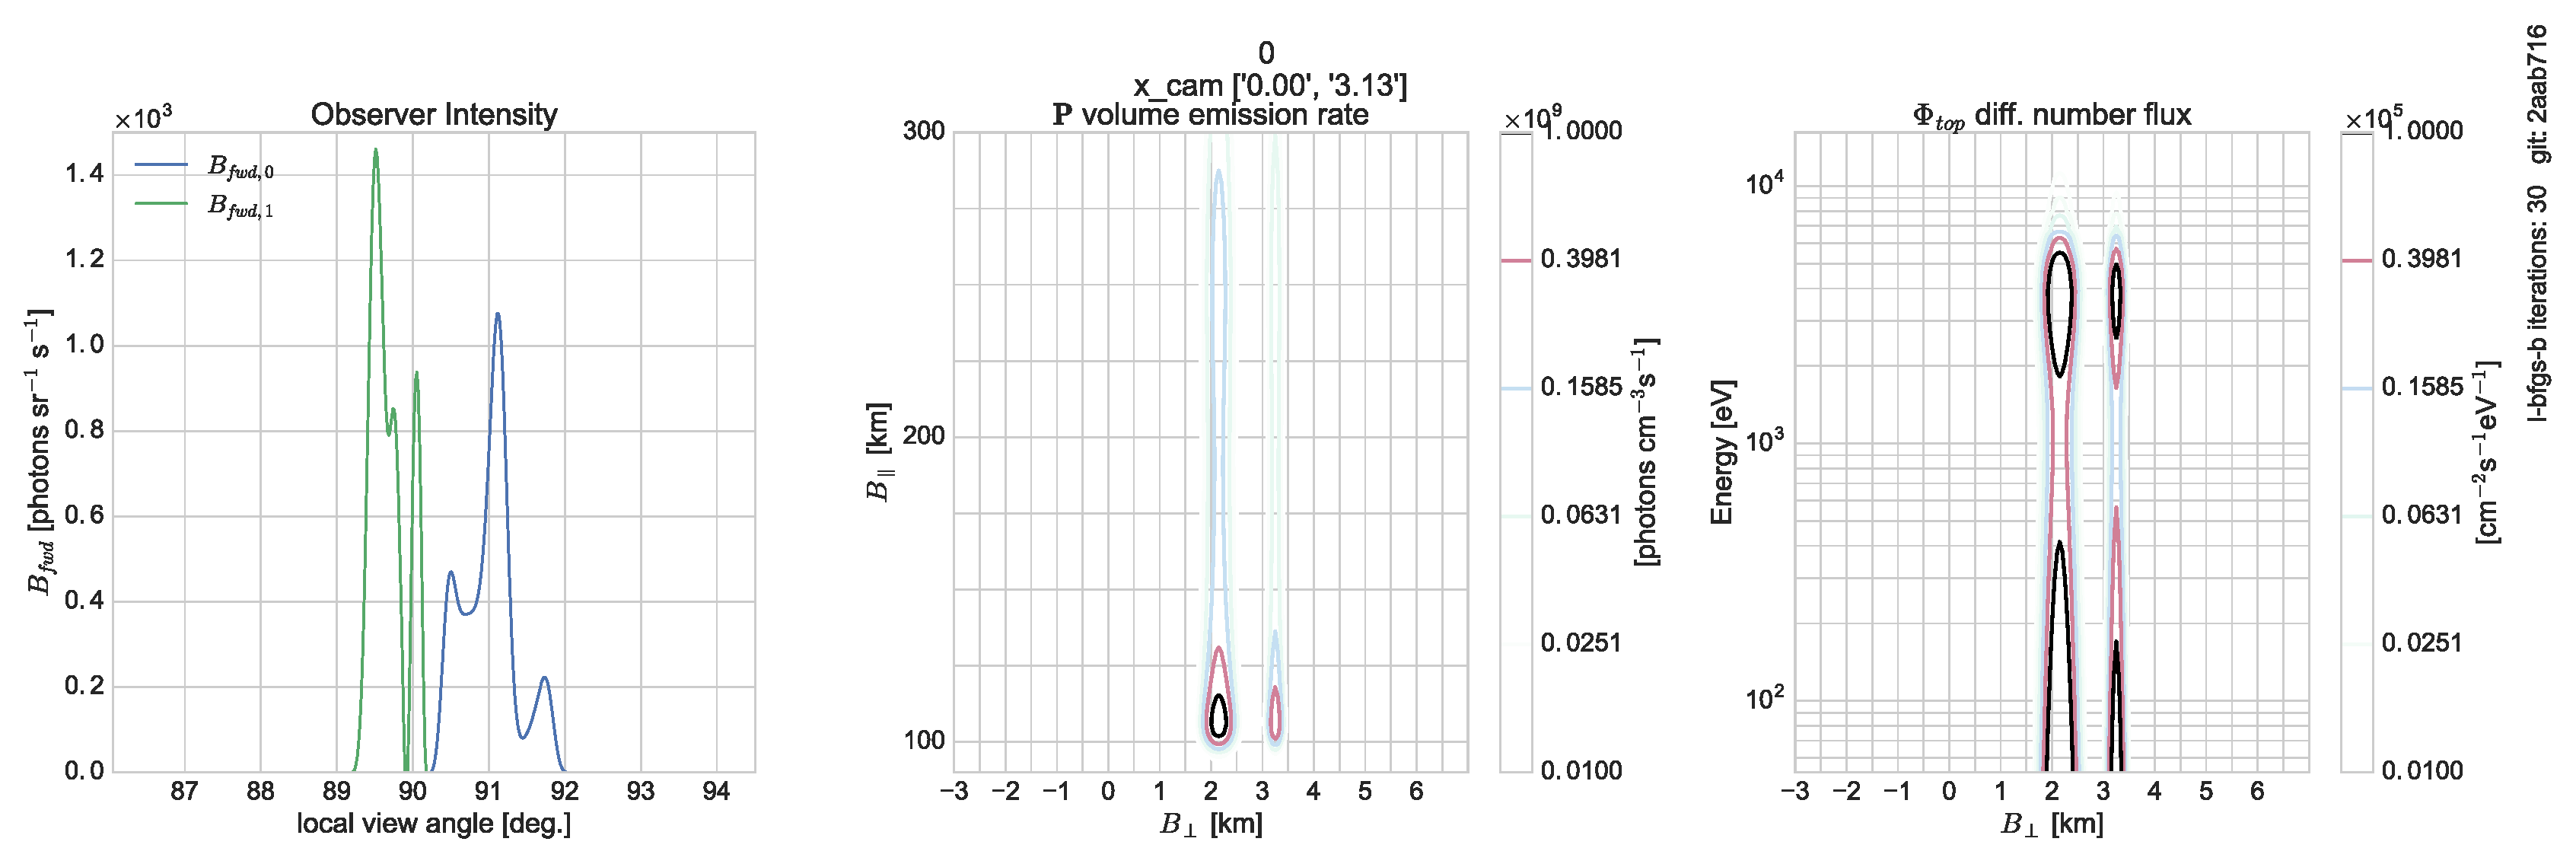
\includegraphics[width=0.9\columnwidth]{gfx/fwd0}
    \caption{Forward model of aurora for HiST two-camera deployment at PFRR. Splitting arc is simulated. 
    	Panel (a) shows ground-observed optical intensity after filtering and wavelength-dependent atmospheric attenuation. 
    	(b) shows the auroral optical volume emission rate vs. $B_\perp$. 
    	(c) shows the unobservable primary electron differential number flux at the ``top'' of the ionosphere, this is the quantity the HiST system estimates with high spatiotemporal resolution.}\label{fig:histfwd}
\end{sidewaysfigure}
\begin{sidewaysfigure}\centering
    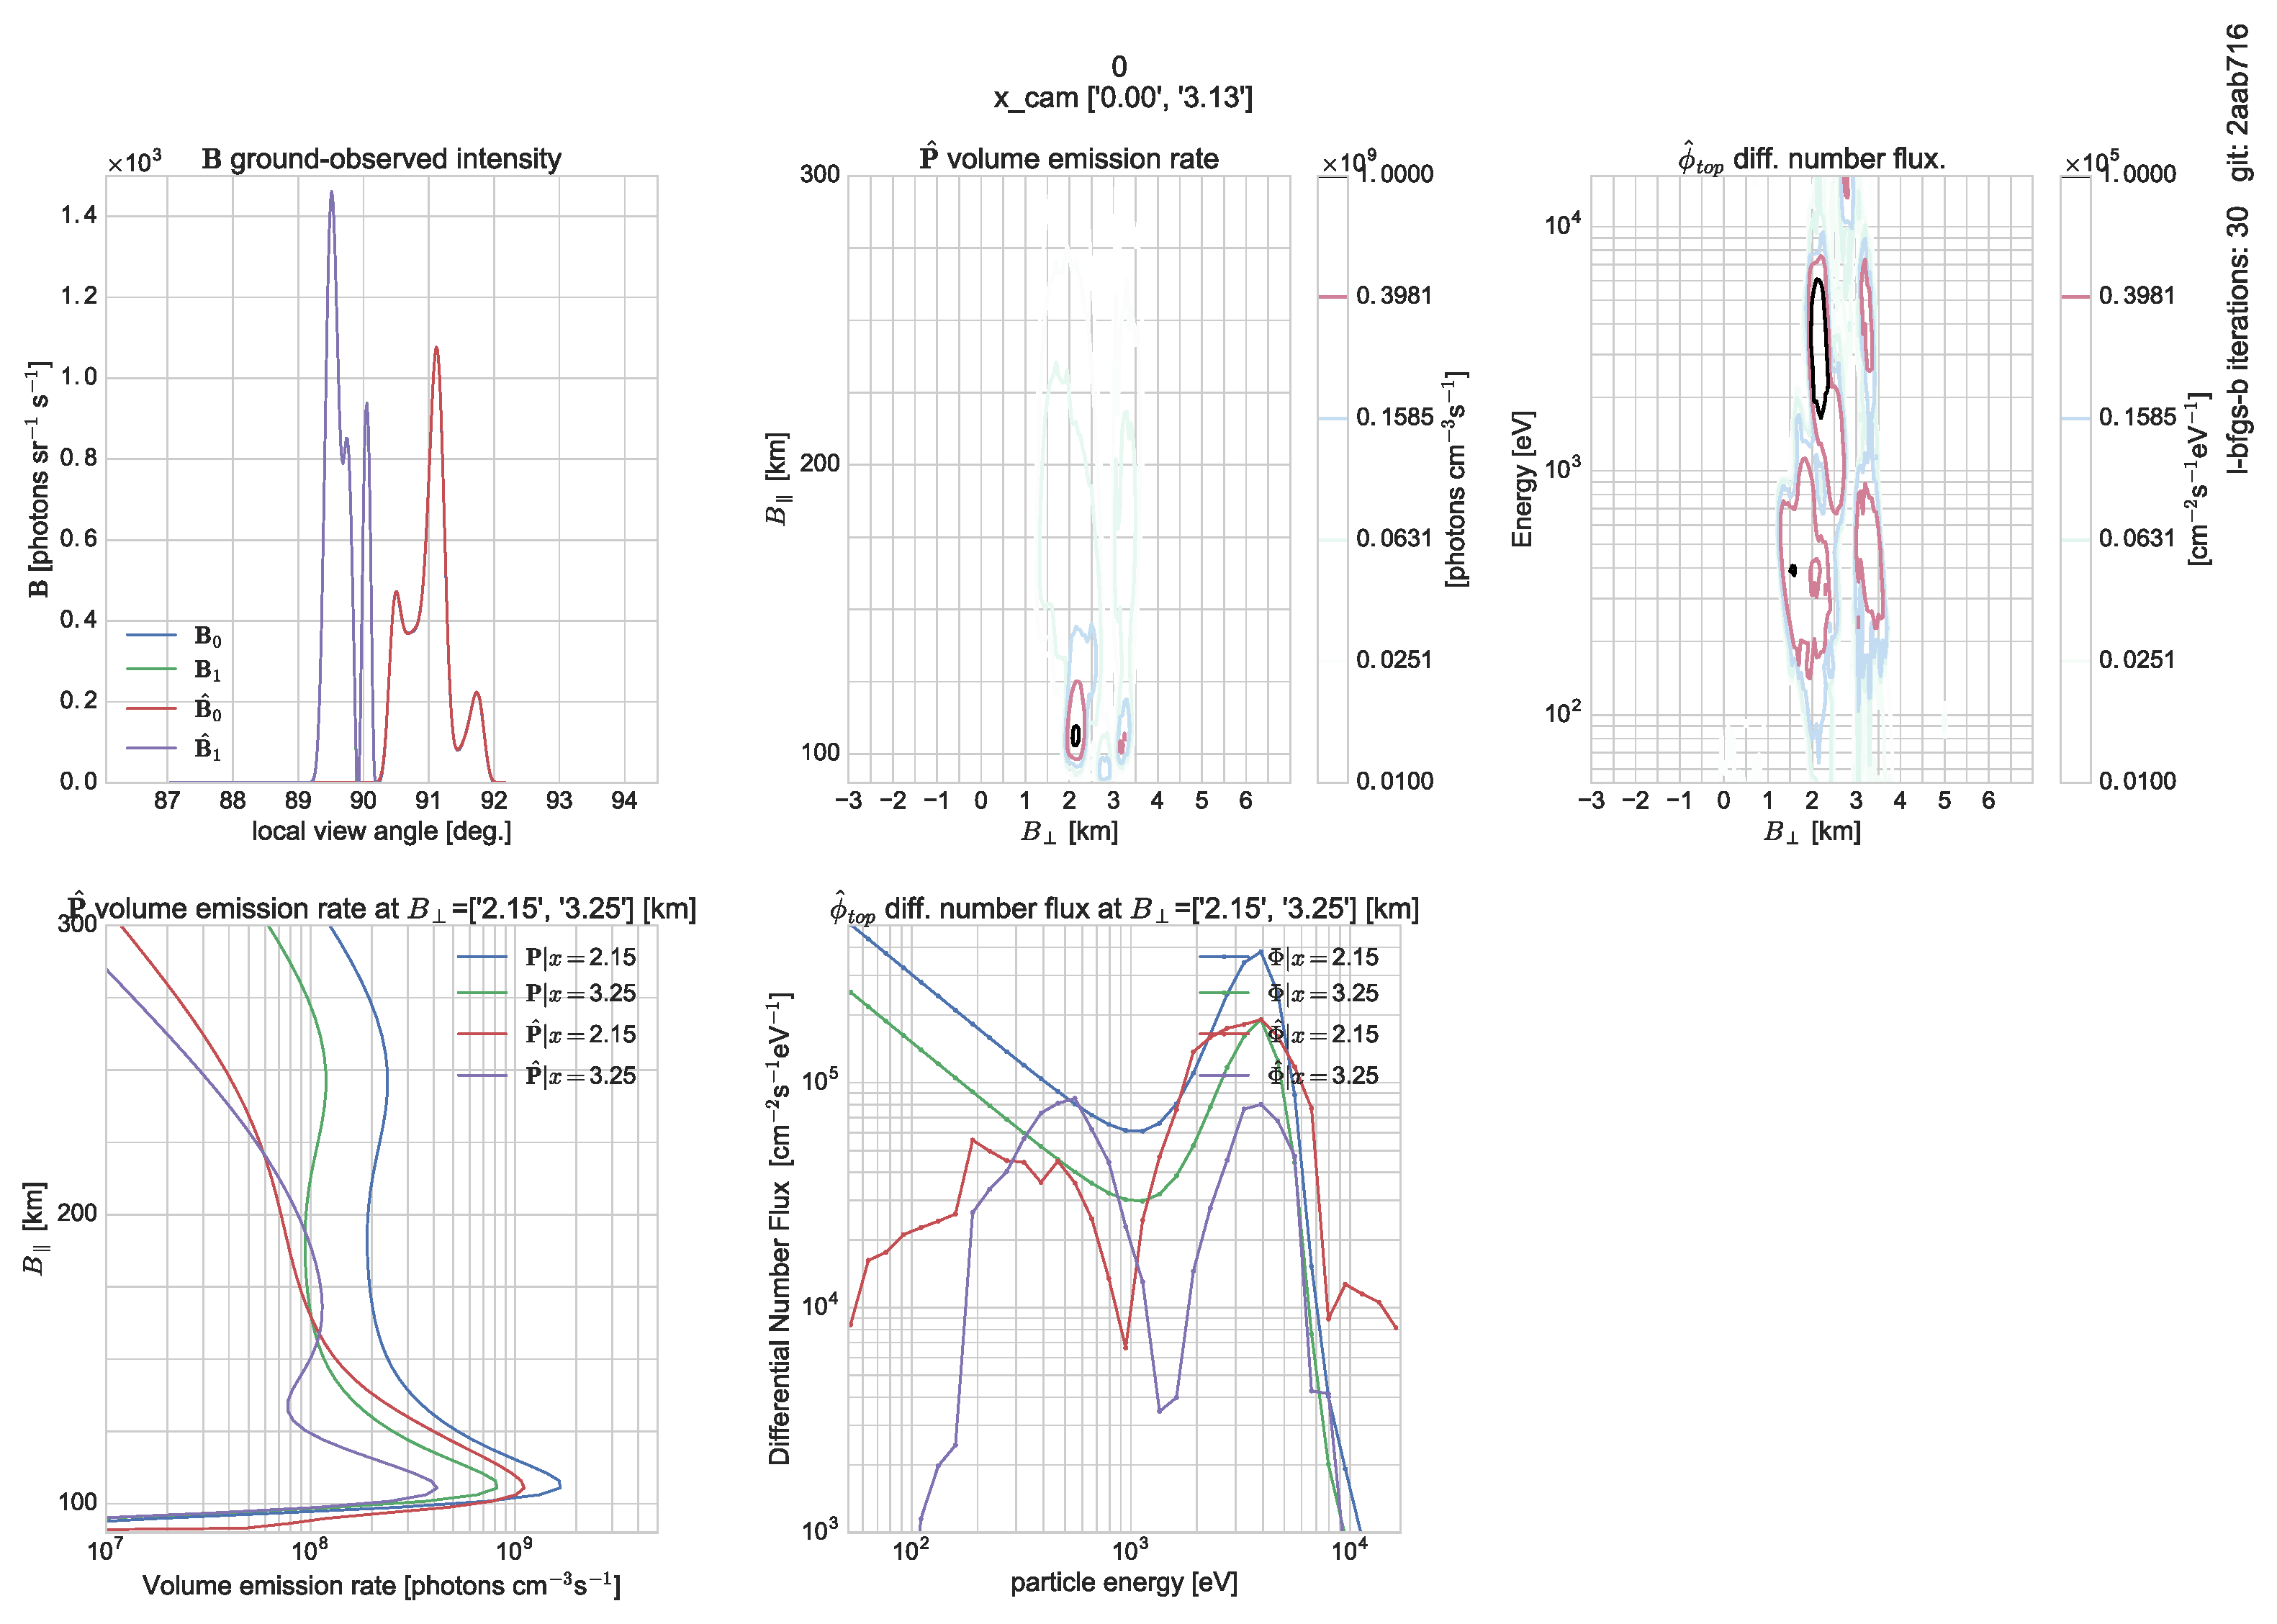
\includegraphics[width=0.75\columnwidth]{gfx/est0}
    \caption{Data inversion for forward modeled HiST two-camera deployment at PFRR. Splitting arc is simulated as in Figure~\ref{fig:histfwd} and precipitation estimated. Panel (a) shows ground-observed and estimated optical intensity after filtering and wavelength-dependent atmospheric attenuation. (b) shows the estimated auroral optical volume emission rate vs. $B_\perp$. (c) shows the estimated primary electron differential number flux at the ``top'' of the ionosphere. (d) shows a 1-D vertical cut of volume emission rate for the two arcs, forward model and estimated. (e) shows a 1-D cut in $B_\perp$ for each arc, forward model and estimated differential number flux.}\label{fig:histest}
\end{sidewaysfigure}